\chapter{Background}
\label{chpt:background}

\epigraph{\textit{“At the heart of quantum mechanics is a rule that sometimes governs politicians or CEOs - as long as no one is watching, anything goes.” }}{Lawrence M. Krauss
}

\section{Weird Vector things}\label{TheBasics}

In this section we will introduce quantum mechanics and its basic unit of information, the qubit, for those with little background in physics. Some knowledge of linear algebra may prove useful and any interested reader should first review basic linear algebra at (REF).
In classical computing and information theory the fundamental unit of information is the familiar bit. Every bit is a binary number 0 or 1 that we use to represent false or true, or combine together to encode any information we wish. We can (for reasons that will become clear) represent 
the classical bit as a 2-dimensional vector where the value 0 or 1 are assigned orthogonal basis vectors,
\begin{equation}
0 = \begin{pmatrix} 1\\ 0 \end{pmatrix},
1 = \begin{pmatrix} 0\\ 1 \end{pmatrix}.
\end{equation}
When discussing the classical bit, this representation has no advantage since 0 and 1 are the only two values a bit can take. However, this 

We can combine single bits in vector form to represent any register of bits,
\begin{equation}
\begin{pmatrix} x_0\\ x_1 \end{pmatrix} \otimes
\begin{pmatrix} y_0\\ y_1 \end{pmatrix}
= \begin{pmatrix} x_0 y_0 \\ x_0 y_1 \\ x_1 y_0 \\ x_1 y_1 \end{pmatrix}.
\end{equation}
This notation captures the relevant information but appears rather unwieldy compared to the equivalent binary or decimal representations.
In this form we write the decimal value 6 as,
\begin{equation}
6_{10} = 110_2 =  \begin{pmatrix} 0\\ 1 \end{pmatrix} \otimes \begin{pmatrix} 0\\ 1 \end{pmatrix} \otimes \begin{pmatrix} 1\\ 0 \end{pmatrix} = \begin{pmatrix} 0 \\ 0 \\ 0 \\ 0 \\ 0 \\ 0 \\ 1 \\ 0 \end{pmatrix}.
\end{equation}
Note that we have a zero in every entry apart from the one corresponding the the decimal 6.
The fundamental operation we can perform on this register is flipping the value of the nth bit i.e. we perform a logical NOT operation $ X \begin{pmatrix} 1\\ 0 \end{pmatrix}  $ to find $ \begin{pmatrix} 0\\ 1 \end{pmatrix} $. 
The matrix X has the form,
\begin{equation}
\begin{pmatrix}
 0 & 1 \\ 1 & 0 
\end{pmatrix}.
\end{equation}
This can be extended to find a matrix that allows us to change any basis state into any other, and therefore we can represent all quantum operations in matrix form. Note also that the not operation is reversible; no information is lost in applying it as many times as we like. This turns out to be a general feature of logical operations in quantum computing.


Adding together numbers in either their binary or decimal form is obvious, however this clearly does not correspond to simple addition in their vector representation. 
\begin{equation}
    6_{10} + 5_{10} = 110_2 + 101_2 \neq  \begin{pmatrix} 0 \\ 0 \\ 0 \\ 0 \\ 0 \\ 0 \\ 1 \\ 0 \end{pmatrix} + \begin{pmatrix} 0 \\ 0 \\ 0 \\ 0 \\ 0 \\ 1 \\ 0 \\ 0 \end{pmatrix}.
\end{equation}
A vector representation of our bits however \textit{should} allow addition and we will now see how to interpret this. Rather than our register being in a definite single \textit{state} corresponding to a single decimal number we can allow superpositions of vectors with each element corresponding to a bit register. For example,
\begin{equation}
    \begin{pmatrix} 0 \\ 1 \\ 0 \\ 0 \end{pmatrix} + \begin{pmatrix} 0 \\ 0 \\ 0 \\ 1  \end{pmatrix},
\end{equation}
is a valid state (however we are now moving away from classical information). This no longer has a clear and unambiguous representation in binary. Furthermore, we can change the signs between vectors and have,
\begin{equation}
    \begin{pmatrix} 0 \\ 1 \\ 0 \\ 0 \end{pmatrix} - \begin{pmatrix} 0 \\ 0 \\ 0 \\ 1  \end{pmatrix}.
\end{equation}
What this represents in information terms is no longer obvious and, more importantly, how can we retrieve information stored in this way? Classically the state of an entire computer is in principle represented by a single string of bits and we can determine this string with certainty. Moving beyond classical information the situation becomes more complicated. If we attempt to measure a superposition of our vectors, asking ``\textit{which state is our register in?}'' we will find $\begin{pmatrix}  0 \\ 1 \\ 0 \\ 0 \end{pmatrix}$ with probability $0.5$ and $\begin{pmatrix}  0 \\ 0 \\ 0 \\ 1 \end{pmatrix}$ with probability 0.5. In order to ensure our probabilities sum to 1 we should normalise our even superposition with a factor of $\frac{1}{\sqrt{2}}$ however this will be ignored for clarity. We can even allow superpositions with more elements i.e. three or more possible outcomes from measurement and factors in front of each vector to adjust the probabilities. To further complicate things we can even allow complex factors in front of our basis vectors, and as it turns out this necessary to fulfil the condition that we can continuously transform any vector into another \cite{hardy2001quantum}. That is to say that there exists a matrix like X introduced above that allows us to move between any states or superpositions thereof. 


So far we have mainly dealt with vectors more complicated than the simple representations of 0 and 1 we introduced earlier. Returning to these we can now introduce the qubit,
\begin{equation}
    \alpha \begin{pmatrix}  1\\ 0 \end{pmatrix} + \beta \begin{pmatrix} 0\\ 1 \end{pmatrix}
\end{equation}
where $\alpha$ and $\beta$ are real or complex number such that $|\alpha|^2 + |\beta|^2 = 1$. This is the reasonable requirement that probabilities should always sum to 1, but encapsulates the principle of superpositions that we measure to find outcomes. In more standard notation we represent vectors in quantum mechanics with a `ket' $|\psi\rangle$. Anything inside the ket is simply a label and can be changed for convenience depending on the situation. For example we traditionally use $\psi$ to denote an arbitrary quantum state with basis vectors in binary i.e.,
\begin{equation}
    |\psi\rangle = \alpha \begin{pmatrix}  1\\ 0 \end{pmatrix} + \beta \begin{pmatrix} 0\\ 1 \end{pmatrix} = \alpha |0\rangle + \beta |1\rangle ,
\end{equation}
is the same state as above in dirac notation. The probability of obtaining the outcome $|1\rangle$ from this state is $|\langle 1|\psi\rangle|^2$ where $\langle 1|$ is known as a `bra,' forming a dirac `bracket' with the state $|\psi\rangle.$ This is nothing more than the inner product of vectors taken to the absolute value squared to ensure we always obtain real and positive probabilities. 

A full model of computation requires more than representations of states and a conceptual method for reading out data. In the next section we will see how to process quantum information in the so-called circuit model. 


A complete mathematical description of quantum mechanics is given in \autoref{Advancedtopics}. 


I have made a list of things that are mentioned several times in the guide that should probably just be introduced here properly: 


Registers
Unitary
Projective Measurement
Adjoints
Oracle
Hadamard
X, Y, Z
Entanglement
Normalisation
Complex phase
Tensor product of gates

(I introduce some of these in Appendix but I think they are to crucial to the readers understanding to be in the appendix.)



A reference table of gates and their matrix representation on one qubit


\section{The gate model and quantum circuits}

introduce in text and table
Cnot coherent classical XOR non separable can't write as a tensor product.
Clifford + T gateset 

This section briefly reviews the gate model for circuit based quantum computing and discusses the similarities between  digital and quantum computers. The gate model is one of the most popular architectures for quantum computation at the moment. A number of companies such as, \textit{Intel \cite{intelqcomp} IBM \cite{ibmqweb}, Google \cite{googleqai} and Rigetti \cite{rigetti}} are all using the gate model approach for quantum computing. There are other architectures for quantum computing however we think that the gate model is the most similar to digital computers.

Both forms of computation follow the same structure, you start with bits (or qubits), operations are performed on the (qu)bits and then you measure the new values of the (qu)bits. We show an example in \autoref{fig:basicoperation}.

%%%% digital circuit
\begin{figure}[H] 
\centering
\begin{subfigure}[h]{0.4\textwidth}
\begin{align*}
\Qcircuit @C=0.5cm @R=0.7cm
{&\lstick{A} &\multigate{2}{Operation} & \\
&\lstick{B} &\ghost{Operation} & \\
&& &\qw &\lstick{Q} \\}
\end{align*}
\caption{Digital operation}
\label{fig:digitalcirc}
\end{subfigure}
~
%%%% Q circuit
\begin{subfigure}[H]{0.4\textwidth}
\begin{align*}
\Qcircuit @C=0.5cm @R=0.7cm
{&\lstick{A} &\multigate{2}{Operation} &\qw &\lstick{A} \\
&\lstick{B} &\ghost{Operation} &\qw &\lstick{B} \\
&\lstick{Q} &\ghost{Operation} &\qw &\lstick{Q} \\}
\end{align*}
\caption{Quantum operation}
\label{fig:quantumcirc}
\end{subfigure}
\caption{Digital and quantum logic circuits for implementing an arbitrary operation on bits $A, B$ returning value $Q$}
\label{fig:basicoperation}
\end{figure}

One of the main differences between the two figures is that in the quantum circuit the inputs $A \& B$ exist after the operation and the output $Q$ is present before the operation. This is a feature of quantum computing being reversible (unitary).  

One of the requirements for quantum computing to be universal is that we are able to perform any single qubit and a single two qubit gate. Most quantum algorithms make use of a Hadamard gate at the beginning of the computation. 


\begin{figure}[H]
    \begin{align*}
    \Qcircuit @C=0.5cm @R=0.7cm
    {&\lstick{0} &\gate{H} &\qw &\rstick{\frac{0+1}{\sqrt{2}}} \\ 
    &\lstick{A} &\qw &\qw &\rstick{A} }
    \end{align*}
    \caption{Hadamard gate acting on the top qubit and no gate performed on the bottom qubit}
    \label{fig:my_label}
\end{figure}


Multiple qubits gates are of the form, control-\textit{Operation}, one of the most popular two-qubit gates used is the Controlled-NOT. The control means use the value of the first qubit to decide whether or not to perform the operation on the target qubit. 


\begin{figure}[H]
    \begin{align*}
    \Qcircuit @C=0.5cm @R=0.7cm
    {&\lstick{0} &\gate{H} &\qw &\rstick{0 \text{  if  } A=0, \frac{0+1}{\sqrt{2}} \text{  if  } A=1 } \\ 
    &\lstick{A} &\ctrl{-1} &\qw &\rstick{A} }
    \end{align*}
    \caption{Hadamard gate acting on the top qubit and no gate performed on the bottom qubit}
    \label{fig:my_label}
\end{figure}



\subsubsection{Digital logic}

Every digital computing operation can be built up from NAND logic gates \cite{sheffer1913set}. We can call a NAND logic gate a universal gate for computation. The NOR gate is also universal in the same way any computation can be constructed from NOR gates.

\begin{figure}[H]
  \centering
  \begin{subfigure}[h]{0.4\textwidth}
  \centering
  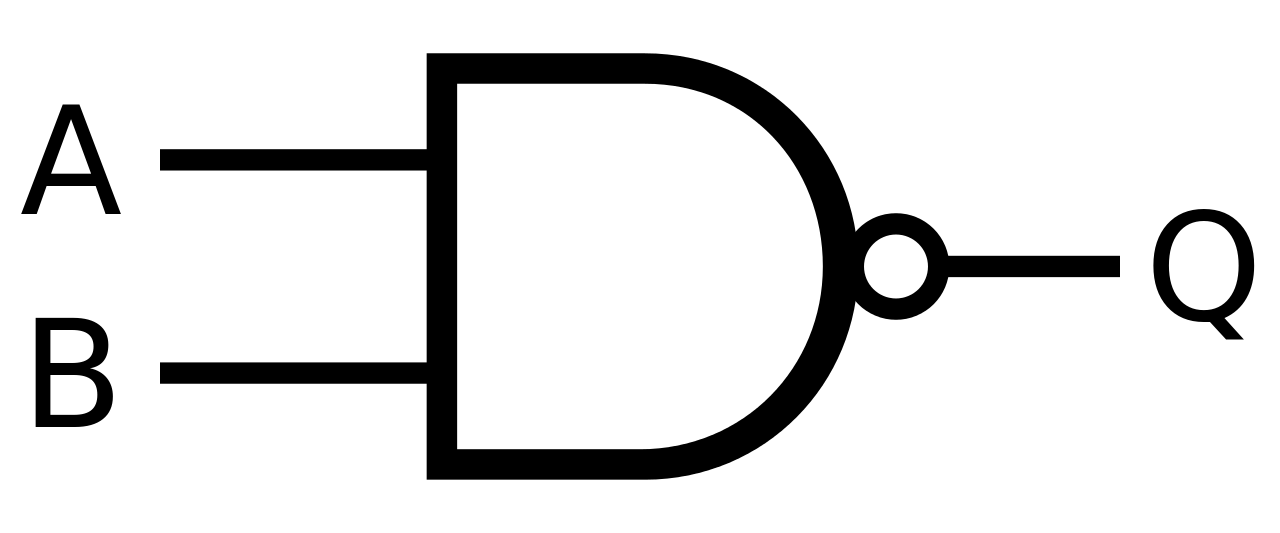
\includegraphics[width=0.7\textwidth]{NAND_ANSI_Labelled_svg.png}
  \caption{The NAND logic gate \cite{nandwiki}.}
  \label{fig:NAND}
\end{subfigure}
~
  \begin{subfigure}[h]{0.4\textwidth}
  \centering
  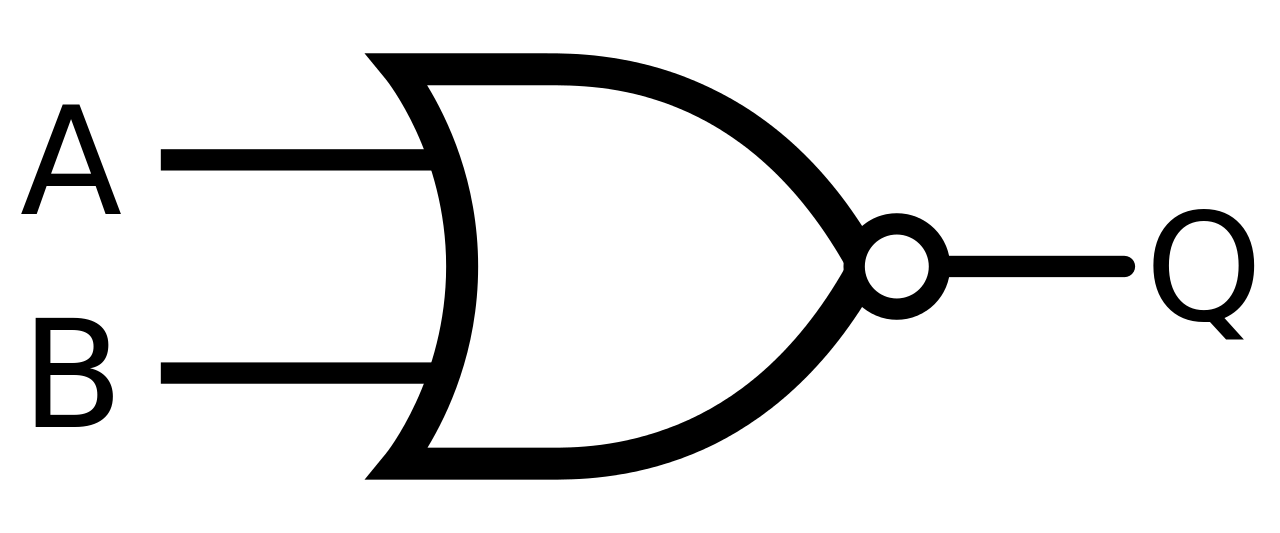
\includegraphics[width=0.7\textwidth]{NOR_ANSI_Labelled_svg.png}
  \caption{The NOR logic gate \cite{norwiki}.}
  \label{fig:NOR}
  \end{subfigure}
\end{figure}

\begin{table}[!htb]
    \caption{Global caption}
    \begin{subtable}{.5\linewidth}
      \centering
        \begin{tabular}{|l|l||l|}
        \hline
        Input A & Input B & Output Q \\ \hline
        0       & 0       & 1       \\ 
        0       & 1       & 0       \\ 
        1       & 0       & 0       \\ 
        1       & 1       & 0       \\
        \hline
    \end{tabular}
    \caption{NOR gate truth table}
    \end{subtable}
    %
    \begin{subtable}{.5\linewidth}
      \centering
        \begin{tabular}{|l|l||l|}
        \hline
        Input A & Input B & Output Q \\ \hline
        0       & 0       & 1       \\ 
        0       & 1       & 1       \\ 
        1       & 0       & 1       \\ 
        1       & 1       & 0       \\
        \hline
    \end{tabular}
    \caption{NAND gate truth table}
    \end{subtable} 
\end{table}


\begin{comment}
reversible logic




%%%%%%%%% circuit 1 
\begin{figure}[h!]
\begin{align*}
\Qcircuit @C=0.5cm @R=0.7cm
{%1
&\lstick{S_1} &\gate{H} &\ctrl{1} &\qw \\
%0
&\lstick{S_0} &\ctrl{-1} &\targ &\qw \\}
\end{align*}
\caption{Schur transform for 2 qubits}
\label{cir:vanilla2}
\end{figure}

\end{comment}